\documentclass[a4paper, 11pt]{report}

\usepackage[utf8]{inputenc}                                                      
\usepackage[french]{babel}                                                       
\usepackage[T1]{fontenc}  
\usepackage[pdftex]{graphicx}                                                    
\usepackage{url}                                                                 
\usepackage{longtable}
\usepackage[bookmarks, 
	colorlinks=false, 
	pdfborder={0 0 0},
	pdftitle={Medicagenda}, 
	pdfauthor={Knop Florian, Kriwin Paul, Placentino Simon},
	pdfsubject={Medicagenda},           
pdfkeywords={UML, ISO/IEC 19505-1:2012, Medicagenda, Projet, analyse, ESI}]{hyperref}   

\newcommand{\HRule}{\rule{\linewidth}{0.5mm}}    

\begin{document}
\begin{titlepage}
	\begin{center}

		
\includegraphics[keepaspectratio=true,width=0.20\textwidth]{ressources/logo}\\[1cm]

		\textsc{\LARGE H.E.B. Ecole Superieur d'Informatique}\\[1.5cm]

		\textsc{\Large Laboratoire d'analyse : Projet d'analyse}\\[0.5cm]

		\HRule \\[0.4cm]
		{\huge \bfseries Medicagenda \\[0.4cm]}
		\HRule \\[1.5cm]

		\noindent
		\begin{minipage}[t]{0.4\textwidth}
			\begin{flushleft} \large
				\emph{Auteurs:}\\
				Florian \textsc{Knop} \href{mailto:39310@heb.be}{39310@heb.be}\\
				Paul \textsc{Kriwin} \href{mailto:39171@heb.be}{39171@heb.be}\\
				Simon \textsc{Placentino} \href{mailto:39631@heb.be}{39631@heb.be}\
			\end{flushleft}
		\end{minipage}%
		\begin{minipage}[t]{0.4\textwidth}
			\begin{flushright} \large
				\emph{Titulaire du cours:} \\
				Mr.~Nicolas \textsc{Pettiaux}
				\href{mailto:npettiaux@heb.be}{npettiaux@heb.be}
			\end{flushright}
		\end{minipage}

		\vfill

		{\large \today}

	\end{center}
	\clearpage\null\newpage
\end{titlepage}

\tableofcontents

\chapter{Modèle conceptuel des données}

\section{Introduction}

\subsection{Objectifs du document}

Cette section sert à documenter et valider les éléments persistants qui devront
être stockés dans le système informatique de la gestion de calendriers de médecins.

\subsection{Domaine de définition du document}

Cette section reprend la description du diagramme métier (diagramme de classes) de la gestion de 
calendriers de médecins.

\subsection{Définitions, acronymes et abréviations}

\begin{enumerate}

\item \texttt{INAMI} : Institut national d'assurance maladie invalidité.

\end{enumerate}

\subsection{Références}

Énoncé du travail de synthèse sur la gestion de calendriers de médecins.

\newpage
\section{Diagramme(s) de classe(s)}

\begin{figure}[hb]
    \centering
    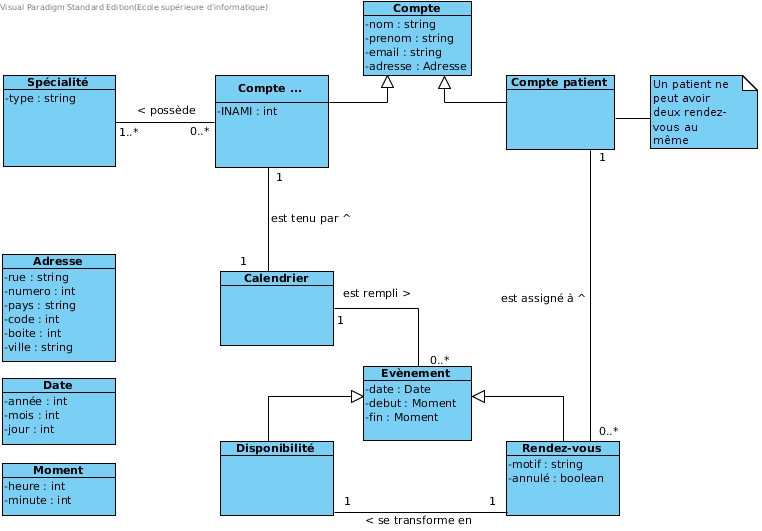
\includegraphics[scale=0.4]{MCD/MCD.jpg}
    \caption{Diagramme de classes Medicagenda}
\end{figure}

\newpage
\section{Classe(s)}


\subsection{Adresse}

\subsubsection{Définition}

Une adresse représente l'adresse postale d'une personne physique.

\subsubsection{Identifiant}

Tous les attributs d'une adresse forment un identifiant.

\subsubsection{Attributs}

\begin{itemize}
    \item rue
    \item numéro
    \item ville
    \item pays
    \item code (= code postal)
    \item boite (optionnel)
\end{itemize}

\subsubsection{Contraintes d'intégrité}

Aucune.

\subsection{Calendrier}

\subsubsection{Définition}

Le calendrier représente tous les évènements futurs et permet
au médecin d'organiser ces évènements. \\
Un client peut ajouter un rendez-vous au calendrier d'un médecin.

\subsubsection{Identifiant}

Mèdecin.INAMI

\subsubsection{Attributs}

Aucun.

\subsubsection{Contraintes d'intégrité}

Aucune.

\subsubsection{Condition de création / suppression d'un objet ou de la classe}

A la création d'un compte médecin, un calendrier est créé pour ce médecin. 
Il n'est pas supprimé.


\subsection{Compte}

\subsubsection{Définition}

Un compte représente un compte sur le site en ligne. Un compte permet la gestion 
d'un calendrier ainsi que des paramètres personnels du client. \\
\texttt{Compte} est la super classe\footnote{selon le principe d'héritage de
l'Orienté Objet} de \texttt{Compte client} et \texttt{Compte Mèdecin}. 

\subsubsection{Identifiant}

Compte.e-mail

\subsubsection{Attributs}

\begin{itemize}
    \item Nom
    \item Prénom
    \item E-mail
    \item Adresse
\end{itemize}

\subsubsection{Contraintes d'intégrité}

Aucune.

\subsubsection{Condition de création / suppression d'un objet ou de la classe}

Un compte est créé par un médecin pour un client, ou par un médecin pour lui-même
ou par un client pour lui-même.
Une fois créé, il n'y a pas de possibilité de suppression.


\subsection{Compte médecin}

\subsubsection{Définition}

Un compte médecin est un type de compte permettant au médecin de gérer ses rendez-vous et disponibilités
grâce au \texttt{calendrier}.

\subsubsection{Identifiant}

Identifiant de \texttt{Compte}.

\subsubsection{Attributs}

Attributs de \texttt{Compte}.

\subsubsection{Contraintes d'intégrité}

Aucune.

\subsubsection{Condition de création / suppression d'un objet ou de la classe}

Voir \texttt{Compte}.

\subsection{Compte patient}

\subsubsection{Définition}

Un compte client est un type de compte permettant au client d'ajouter des rendez-vous avec un médecin.
Un client peut modifier ses paramètres dans son espace client.

\subsubsection{Identifiant}

Identifiant de \texttt{Compte}.

\subsubsection{Attributs}

Attributs de \texttt{Compte}.

\subsubsection{Contraintes d'intégrité}

Aucune.

\subsubsection{Condition de création / suppression d'un objet ou de la classe}

Voir \texttt{Compte}.

\subsection{Date}

\subsubsection{Définition}

Une date représente une date représentée par un jour, un mois et une année.

\subsubsection{Identifiant}

Date.jour + Date.mois + Date.année

\subsubsection{Attributs}

\begin{itemize}

    \item{jour}
    \item{mois}
    \item{année}

\end{itemize}

\subsubsection{Contraintes d'intégrité}

\begin{itemize}
    \item Un jour prend les valeurs entre 1 et 31.
    \item Un mois prend les valeurs entre 1 et 12.
    \item La valeur maximale du jour dépend du mois (30 / 31 / 28 / 28).
\end{itemize}

\subsubsection{Condition de création / suppression d'un objet ou de la classe}

\subsection{Disponibilité}

\subsubsection{Définition}

Une disponibilité est une plage horaire dans laquelle un médecin accepte
des nouveaux rendez-vous.

\subsubsection{Identifiant}

Événement.date + Événement.début + Événement.fin

\subsubsection{Attributs}

Voir \texttt{Événement}.

\subsubsection{Contraintes d'intégrité}

Voir \texttt{Événement}.

\subsubsection{Condition de création / suppression d'un objet ou de la classe}

Une disponibilité est créée lorsqu'un médecin décide d'accepter de nouveaux rendez-vous ou quand un
rendez-vous a été annulé par un client. Dans ce cas, le rendez-vous est transformé en disponibilité.

\subsection{Événement}

\subsubsection{Définition}

Un évènement est un horaire pendant lequel le médecin peut recevoir un patient ou en accepter de nouveaux.

\subsubsection{Identifiant}

Événement.date + Événement.début + Événement.fin

\subsubsection{Attributs}

\begin{itemize}
    \item date
    \item début
    \item fin
\end{itemize}

\texttt{début} et \texttt{fin} représentent des heures/minutes de début et fin d'un évènement.

\subsubsection{Contraintes d'intégrité}

$fin > début$.

\subsubsection{Condition de création / suppression d'un objet ou de la classe}

Un évènement est soit créé par un médecin, soit par un client. Une fois l'évènement passé,
il est stocké dans la base de données.

\subsection{Moment}

\subsubsection{Définition}

Un moment est représenté par une heure et des minutes.

\subsubsection{Identifiant}

Moment.heure + Moment.minute

\subsubsection{Attributs}

\begin{itemize}
    \item{heure}
    \item{minute}
\end{itemize}

\subsubsection{Contraintes d'intégrité}

\begin{itemize}
    \item heure doit être compris entre 0 et 23.
    \item minute doit être compris entre 0 et 59.
\end{itemize}

\subsubsection{Condition de création / suppression d'un objet ou de la classe}

\subsection{Rendez-vous}

\subsubsection{Définition}

Un rendez-vous est un horaire créé par le client ou par le médecin où le client se doit 
d'assister à la séance.
Un rendez-vous peut être annulé avant la date de ce dernier par le client lui-même.

\subsubsection{Identifiant}

Événement.date + Événement.début + Événement.fin

\subsubsection{Attributs}

\begin{itemize}
    \item motif
    \item annulé
\end{itemize}

\subsubsection{Contraintes d'intégrité}

Aucune

\subsubsection{Condition de création / suppression d'un objet ou de la classe}

Un rendez-vous est créé soit par le médecin, soit par le client. Il n'est jamais supprimé.

\subsection{Spécialité}

\subsubsection{Définition}

Une spécialité définit le type d'activité médicale qu'effectue le médecin.

\subsubsection{Identifiant}

Spécialité.type

\subsubsection{Attributs}

\begin{itemize}
    \item type
\end{itemize}

\subsubsection{Contraintes d'intégrité}

Aucune.

\newpage
\section{Associations}

\subsection{possède \texttt{Compte médecin-> Spécialité}}
\subsubsection{Définition}
Associe des spécialités à un médecin par le biais de son compte.
\subsubsection{Contraintes d'intégrité}
Le médecin ne peut posséder deux fois la même spécialité.

\subsection{tient un \texttt{Compte médecin -> Calendrier}}
\subsubsection{Définition}
Associe un calendrier de disponibilités à un médecin.
\subsubsection{Contraintes d'intégrité}
Il pourrait éventuellement cumuler plusieurs calendriers pour subdiviser ses
rendez-vous.

\subsection{est assigné à \texttt{Rendez-vous -> Compte patient}}
\subsubsection{Définition}
Associe un patient à un rendez-vous.
\subsubsection{Contraintes d'intégrité}
Un patient peut cumuler plusieurs rendez-vous mais jamais au même moment.

\subsection{est rempli de \texttt{Calendrier -> Événement}}
\subsubsection{Définition}
Associe un calendrier à des évènements qui le composent.
\subsubsection{Contraintes d'intégrité}
\texttt{Aucune}

\subsection{Se transforme en \texttt{Disponibilité -> Rendez-vous}}
\subsubsection{Définition}
Associe une disponibilité en tant que rendez-vous.
\subsubsection{Contraintes d'intégrité}
Cette association peut être brisée.
\newpage

\section{Dictionnaire des données}

\begin{center}
\begin{longtable}{|p{2cm}|p{2cm}|p{3cm}|p{2cm}|p{2cm}|p{2cm}|}
		\hline
		Nom & Classe & Définition & Type & Domaine & CI \\
		\hline
		annulé & Rendez-vous & \parbox[t]{3cm}{Vrai si le rendez-vous a été annulé\\} &
        Booléen & Vrai ou faux & Aucune \\
		\hline
        adresse & Compte & \parbox[t]{3cm}{L'adresse du titulaire du compte\\} & Chaîne 
        & \parbox[t]{2cm}{Toutes adresses valables\\} & Aucune \\
        \hline
        année & Date & L'année de la date & Entier & \parbox[t]{2cm}{Aucun\\ domaine particulier\\} & Aucune \\
        \hline
        boite & Adresse & \parbox[t]{3cm}{Le numéro de la boîte postale\\} & Entier & \parbox[t]{2cm}{Aucun\\ domaine particulier\\} &
        Optionnel \\
        \hline
        code & Adresse & \parbox[t]{3cm}{Le code postal\\} & Entier & \parbox[t]{2cm}{Aucun\\ domaine particulier\\} & Aucune \\
        \hline
        date & Événement & \parbox[t]{3cm}{La date de l'évènement\\} & Date & \parbox[t]{2cm}{Aucun\\ domaine particulier\\} &
        Aucune \\
        \hline
        début & Événement & \parbox[t]{3cm}{L'heure de début de l'évènement\\} & Moment & \parbox[t]{2cm}{Aucun\\ domaine particulier\\} &
        Aucune \\
        \hline
        e-mail & Compte & \parbox[t]{3cm}{L'e-mail du titulaire du compte\\} & Chaîne & \parbox[t]{2cm}{Aucun\\ domaine particulier\\}
        & \parbox[t]{2cm}{E-Mail\\ valide} \\
        \hline
        fin & Événement & \parbox[t]{3cm}{L'heure de fin de l'évènement\\} & Moment & \parbox[t]{2cm}{Aucun\\ domaine particulier\\} &
        Aucune \\
        \hline
        heure & Moment & \parbox[t]{3cm}{L'heure du\\moment\\} & Entier & Valeur de 0 à 23 &
        Aucune \\
        \hline
        INAMI & Compte médecin & \parbox[t]{3cm}{Le numéro \\INAMI du médecin\\} & Entier & \parbox[t]{2cm}{Aucun\\ domaine particulier\\}
        & Aucune \\
        \hline
        jour & Date & Le jour de la date & Entier & 1 à 31 & \parbox[t]{2cm}{Valeur \\correcte du jour selon\\ le mois\\} \\
        \hline
        minute & Moment & \parbox[t]{3cm}{La minute de\\ l'heure du\\ moment\\} & Entier & Valeur de 0 à 59 &
        Aucune \\
        \hline
        mois & Date & Le mois de la date & Entier & Valeur de 1 à 12 & Aucune \\
        \hline
        motif & Rendez-vous & \parbox[t]{3cm}{Le motif \\du rendez-vous\\} & Chaîne & \parbox[t]{2cm}{Aucun\\ domaine particulier\\}
        & Aucune \\
        \hline
        nom & Compte & \parbox[t]{3cm}{Le nom du titulaire du compte\\} & Chaîne & \parbox[t]{2cm}{Aucun\\ domaine particulier\\}
        & Aucune \\
        \hline
        numéro & Adresse & \parbox[t]{3cm}{Le numéro dans la rue\\} & Entier & \parbox[t]{2cm}{Nombres positifs} & Aucune \\
        \hline
        pays & Adresse & \parbox[t]{3cm}{Le pays dans\\lequel se situe\\l'adresse\\}  & Chaîne & \parbox[t]{2cm}{Aucun\\ domaine particulier\\}  
        & Aucune \\
        \hline
        prénom & Compte & \parbox[t]{3cm}{Le prénom du titulaire du compte\\} & Chaîne & \parbox[t]{2cm}{Aucun\\ domaine particulier\\}
        & Aucune \\
        \hline
        rue & Adresse & \parbox[t]{3cm}{La rue de\\ l'adresse\\} & Chaîne & \parbox[t]{2cm}{Aucun\\ domaine particulier\\} & Aucune \\
        \hline
        type & Spécialité & \parbox[t]{3cm}{Le type de\\ la spécialité\\} & Chaîne & \parbox[t]{2cm}{Les types\\ valables\\} & Aucune\\
        \hline
        ville & Adresse & \parbox[t]{3cm}{La ville de\\ l'adresse\\} & Chaîne & \parbox[t]{2cm}{Aucun\\ domaine particulier\\} & Aucune \\
        \hline
        
\end{longtable}
\end{center}



\chapter{Modèle conceptuel des traitements}

\section{Introduction}

\subsection{Objectifs du document}
Ce document présente la décomposition fonctionnelle du projet \texttt{Medicagenda}.
\subsection{Domaine de définition du document}
L'ensemble des sous-systèmes décrits dans le M.C.D. :
\begin{itemize}
	\item SS1 : \texttt{Medicagenda}.
\end{itemize}
\subsection{Définitions, acronymes et abréviations}
\begin{itemize}
	\item \texttt{CRUD} :
		\begin{itemize}
			\item[] Create,
			\item[] Read,
			\item[] Update,
			\item[] Delete,
		\end{itemize}
\end{itemize}
\subsection{Références}
\begin{itemize}
	\item[] Etude de cas de l'agenda
		médical\footnote{\href{../Enonce_Travail_Synthese_14-15.pdf}{voir
		étude de cas}}
	\item[] M.C.D. de \texttt{Medicagenda}\footnote{\href{../MCD/MCD.pdf}{voir document M.C.D.}}
\end{itemize}
\newpage
\section{Acteurs}
\subsection{Acteurs externes}
Les acteurs externes au SIA complet du \texttt{Medicagenda} se retrouvent dans le 
diagramme de contexte\footnote{Voir~\ref{dc} Diagramme de contexte} : 
\begin{itemize}
	\item Patient : Personne qui pourra prendre rendez-vous auprès d'un ou
		plusieurs médécins pour une ou plusieurs spécialisations.
\end{itemize}
\subsection{Acteurs internes}
\begin{itemize}
	\item Médecin : Propriétaire de l'agenda pouvant éventuellement être le
		gestionnaire de ce dernier.
\end{itemize}
\subsection{Diagramme des acteurs du SIA}
\begin{figure}[hb]
	\centering
	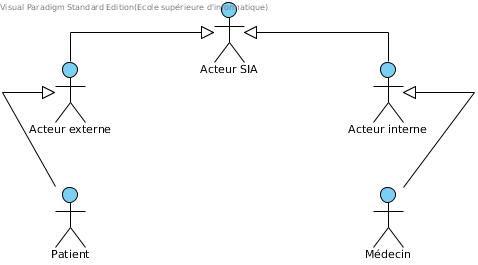
\includegraphics[scale=0.7]{MCT/acteurs.jpg}
	\caption{Diagramme des acteurs du SIA}
	\label{fig:acteurs}
\end{figure}
\newpage
\section{Vision globale du SI}
\subsection{\label{dc}Diagramme de contexte}
Ce diagramme présente tout le système informatique du \texttt{Medicagenda} et les acteurs 
externes avec lesquels il est en relation. 
\begin{figure}[hb]
	\centering
	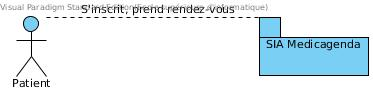
\includegraphics[scale=0.7]{MCT/contexte.jpg}
	\caption{Diagramme de contexte}
	\label{fig:contexte}
\end{figure}
\subsection{Diagramme des systèmes}
\begin{figure}[hb]
	\centering
	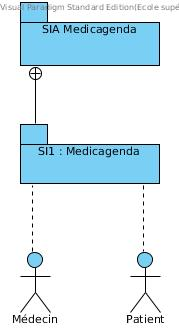
\includegraphics[scale=0.7]{MCT/systemes.jpg}
	\caption{Diagramme des systèmes}
	\label{fig:systemes}
\end{figure}
\newpage
\section{Diagramme des sous-sytèmes}
\begin{figure}[hb]
	\centering
	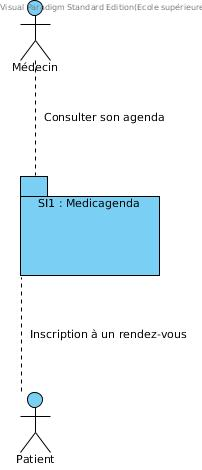
\includegraphics[scale=0.7]{MCT/sous-systeme.jpg}
	\caption{Diagramme des sous-systèmes}
	\label{fig:sous-systeme}
\end{figure}
\newpage
\section{Système SI1 : Agenda}
\subsection{Diagramme des Use Cases}
\begin{figure}[hb]
	\centering
	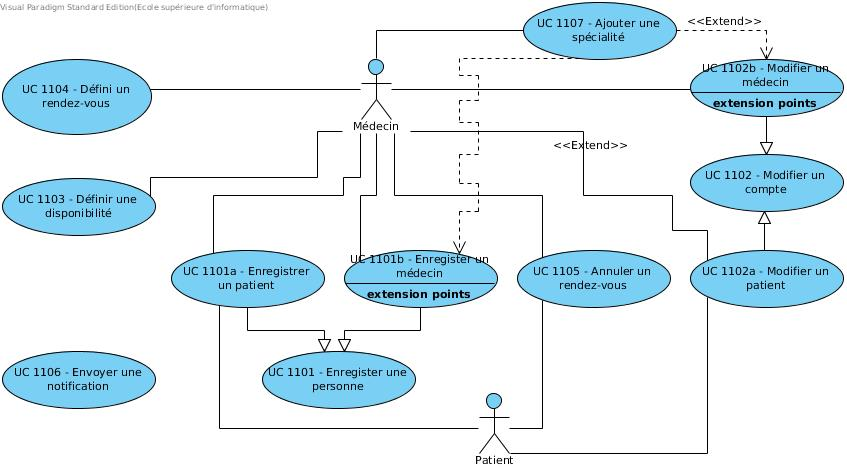
\includegraphics[scale=0.5]{MCT/SS1_UC.jpg}
	\caption{Diagramme des Use Cases}
	\label{fig:ss1_uc}
\end{figure}
\subsection{Description des \texttt{U.C.}}
\subsubsection{1101 Enregistrer une personne}
\paragraph{1101a Enregistrer un patient}
Ce \texttt{U.C.} permet créer un nouveau compte pour un patient qui n'en possède pas au
par avant. Ce enregistrement peut se faire :
\begin{itemize}
	\item directement par le patient lui-même,
	\item directement par le médecin lui-même,
	\item directement par le médecin lui-même lors de la prise de rendez-vous.
\end{itemize}
\paragraph{1101b Enregistrer un médecin}
Ce \texttt{U.C.} permet créer un nouveau compte pour un médecin qui n'en possède pas au
par avant. Ce enregistrement peut se faire :
\begin{itemize}
	\item directement par le médecin lui-même,
	\item par un organisme externe déployant le système (tel que l'INAMI).
\end{itemize}

L'enregistrement d'un nouveau médecin peut entrainer 
\begin{itemize}
	\item l'enregistrement de	spécialités associées à ce dernier ne se trouvant pas déjà dans la 
		BDD\footnote{Base De Données}.
	\item la création d'un nouveau calendrier.
\end{itemize}
Ce \texttt{U.C.} peut donc faire appel au \texttt{U.C. 1107}.
\subsubsection{1102 Modifier un compte}

\paragraph{1102a Modifier un patient}
Ce \texttt{U.C.} permet de modifier les données d'un compte. Cette modification
peut se faire :
\begin{itemize}
	\item par le médecin directement n'intervenant que sur un certain niveau de
		données,
	\item par le patient directement n'intervenant que sur un certain niveau de
		données.
\end{itemize}

Certaines modifications de données, telles que l'annulation d'un rendez-vous par
l'un ou par l'autre, doivent être notifiée.

Le patient peut ainsi s'inscrire à un rendez-vous selon les disponibilités
proposées par le médecin.
\paragraph{1102b Modifier un médecin}
Ce \texttt{U.C.} permet, uniquement au \textbf{médecin} (ou éventuellement à un
service externe tel que l'INAMI) de modifier son compte.

Il peut faire appel aux 
\begin{itemize}
	\item \texttt{~U.C. 1103} 
	\item \texttt{~U.C. 1104} 
	\item \texttt{~U.C. 1105}
	\item \texttt{~U.C. 1107}
\end{itemize}

\subsubsection{\label{1103}1103 Définir une disponibilité}
Ce \texttt{U.C.} permet a un médecin de définir une plage de disponibilité dans
un jour du calendrier. Il permet, aussi, de redéfinir une disponibilité après
l'annulation d'un rendez-vous.
\subsubsection{\label{1104}1104 Définir un rendez-vous}
Ce \texttt{U.C.} permet à un patient de définir un rendez-vous selon le
calendrier d'un médecin en se basant sur l'ensemble de ses disponibilités. 
Ce \texttt{U.C.} peut aussi être effectué par un médecin pour le compte d'un
patient directement si un nouveau rendez-vous doit être fixé.

Le rendez-vous enclenchera l'ajout d'un entrée dans le mécanisme des
notifications.
\subsubsection{\label{1105}1105 Annuler un rendez-vous}
Ce \texttt{U.C.} permet a une disponibilité de l'agenda d'être à nouveau
disponible. L'annulation peut être faite par le patient ou par le médecin. 
\subsubsection{\label{1106}1106 Envoyer une notification}
Ce \texttt{U.C.} \textbf{automatisé} envoie des notifications aux patients ayant
un rendez-vous. Celle-ci sera envoyée à l'heure définie par le patient. Si ce 
dernier n'a pas annulé avant, la consultation lui sera facturée.
\subsubsection{\label{1107}1107 Ajouter une spécialité}
Ce \texttt{U.C.} permet de rajouter des spécialités dans la base de données et
uniquement par un médecin. Cet ajout doit passer par un organisme, tel que
l'INAMI, pouvant le confirmer.
\newpage
\subsection{Matrice CRUD}

Pour la lisibilité de la matrice, cette dernière a été séparée en deux tableaux.
Seuls les \texttt{U.C.} ayant une action avec une des classes du tableau apparaissent.

\begin{center}
	\begin{longtable}{|p{1.5cm}|p{1.5cm}|p{1.5cm}|p{1.5cm}|p{1.5cm}|}
		\hline
		& Compte & Compte Médecin & Compte Patient & Spécialité \\
		\hline
		UC1101a & C & / & C & / \\
		\hline
		UC1101b & C & C & / & R \\
		\hline
		UC1102a & U & / & U & / \\
		\hline
        UC1102b & U & U & / & / \\
        \hline
		UC1105  & R & R & R & R \\
		\hline
		UC1106 & R & R & R & R \\
		\hline
        UC1107 & / & / & / & C \\
        \hline

	\end{longtable}
\end{center}

\begin{center}
	\begin{longtable}{|p{2.2cm}|p{2.2cm}|p{2.2cm}|p{2.2cm}|}
		\hline
		& Évènement & Rendez-vous & Disponibilité  \\
		\hline
		UC1103 & C & R & C \\
		\hline 
		UC1104 & C & C & R \\
		\hline
		UC1105 & U & U & / \\
		\hline
		UC1106 & R & R & / \\
		\hline

	\end{longtable}
\end{center}

\chapter{Use Case Spécification 1104 - Définir un rendez-vous}

\section{Introduction}

\subsection{Objectifs du document}
Ce document présente aux utilisateurs les spécifications fonctionnelles du \texttt{U.C.},
1104, Définir un rendez-vous, (C, R) afin que le médecin puisse le valider.

\subsection{Domaine de définition du document}
La description du \texttt{U.C.} est complète pour les points 2 à 8. Par contre, le
diagramme d’activités se limite à celui qui présente la création d’un nouveau 
rendez-vous (il faudrait y ajouter la suppression d’un rendez-vous). 

\subsection{Définitions, acronymes et abréviations}
Définition INAMI : voir étude de cas et MCD\footnote{\href{../MCD/MCD.pdf}{voir document M.C.D.}}.

\subsection{Références}
\begin{itemize}
	\item[] Étude de cas de l'agenda
		médical\footnote{\href{../Enonce_Travail_Synthese_14-15.pdf}{voir
		étude de cas}}
	\item[] M.C.D. de \texttt{Medicagenda}\footnote{\href{../MCD/MCD.pdf}{voir document M.C.D.}}
	\item[] M.C.T. de \texttt{Medicagenda}\footnote{\href{./MCT.pdf}{voir document M.C.T.}}
\end{itemize}
\newpage

\section{Définition de Use Case}
\subsection{Identifiant et nom}
\texttt{U.C. 1104} - Définir un rendez-vous (C, R).
\subsection{Brève description}
Ce \texttt{U.C.} permet au médecin ou au patient de définir un rendez-vous.
\subsubsection{Définir un rendez-vous}
Cette définition peut se faire
\begin{itemize}
	\item directement par le médecin,
	\item directement par le patient.
\end{itemize}

La définition implique \texttt{l'enregistrement d'un compte patient} si il n'existe pas.
\newpage

\section{Flux}
\subsection{Flux de base}
Le patient commence par s'identifier sur son compte personnel. 
Si son compte n'existe pas, un message apparaitra pour le prévenir et l'inviter
à le créer. Il y aura, si acceptation, affichage des champs obligatoires à
remplir. Après validation et confirmation, il peut s'identifier auprès de la plateforme.
Le patient va, ensuite, sélectionner le médecin auprès duquel il souhaite
prendre rendez-vous à travers une boite de recherche ou un menu déroulant par
ordre :
\begin{itemize}
	\item alphabétique,
	\item de localisation
	\item ou de spécialité.
\end{itemize}

Si celui-ci n'existe pas, un fenêtre apparaitra permettant d'entrer les données 
de ce dernier pour ensuite traiter, par la plateforme, la
demande d'enregistrement auprès du médecin susdit et le patient retourne sur
son menu principal.
Si il existe, le patient choisira, dans l'agenda du médecin, la date qu'il
souhaite. Si cette date ne contient pas de disponibilité souhaitée, ou de
disponibilité souhaitée libre, le patient recherchera une autre date qui le 
convient.
Une fois la disponibilité sélectionnée, il sera demandé d'entrer un commentaire,
ou non à l'attention du médecin. Un message récapitulatif apparaitra dans une
fenêtre demandant d'accepter la demande et les conditions d'annulation.

\subsection{Flux alternatifs}

\subsubsection{Abandon du U.C.}
A tout moment, le patient peut abandonner l'enregistrement du rendez-vous pour
peu qu'il n'ai pas déjà confirmé.
\newpage

\section{Acteurs, mode, performances, exigences particulières}
\subsection{Acteurs}
Patient ou médecin.
\subsection{Mode}
Interactif unitaire.
\subsection{Événement déclencheur}
Le besoin, d'un patient ou d'un médecin, d'établir un rendez-vous chez un
spécialiste.
Techniquement :
\begin{itemize}
	\item depuis le compte d'un médecin,
	\item depuis le compte d'un patient.
\end{itemize}

\subsection{Performance}
\texttt{Sans Objet}
\subsection{Exigences particulières}
\texttt{Sans Objet}
\newpage

\section{Conditions préalables}
\subsection{Création d'un compte patient}
Pour l'associer à un rendez-vous.
\subsection{Création d'un compte médecin}
Pour créer un agenda public.
\subsection{Définition d'une disponibilité}
Pour permettre au patient de créer un rendez-vous.

\section{Conditions postérieures}
Si abandon du \texttt{U.C.}, le système se retrouve dans l'état où il était avant le
lancement du \texttt{U.C.}.
\newpage

\section{Points d'inclusion et d'extension}
\subsection{Extension}
\texttt{Aucune n'a été déduite de l'analyse}.
\subsection{Inclusion}
\texttt{Aucune n'a été déduite de l'analyse}.
\newpage

\section{Règles de gestion}
\subsection{Classes concernées}
\begin{center}
	\begin{longtable}{|p{2.2cm}|p{2.2cm}|p{2.2cm}|p{2.2cm}|}
		\hline
		 Compte patient & Compte médecin & Disponibilité & Rendez-vous \\
		\hline
		 CR & R & RU & C \\
		\hline
	\end{longtable}
\end{center}
\subsection{Validation des encodages de données}
Les données seront conformes aux formats, aux types et aux contraintes définis
dans le M.C.D. Sinon, affichage d’un message (message standard de l'interface) 
demandant la correction avant sauvegarde des données.
En particulier, validation du numéro INAMI encodé par un organisme externe.

\subsection{Messages}
\begin{itemize}
	\item ``Numéro INAMI en attente de validation''
	\item ``Compte patient non existant dans la base de données''
	\item ``Compte médecin introuvable dans la base de données''
	\item ``Données entrées non valides''
\end{itemize}
\newpage

\section{Diagramme d'activités}
\begin{figure}[hb]
	\centering
	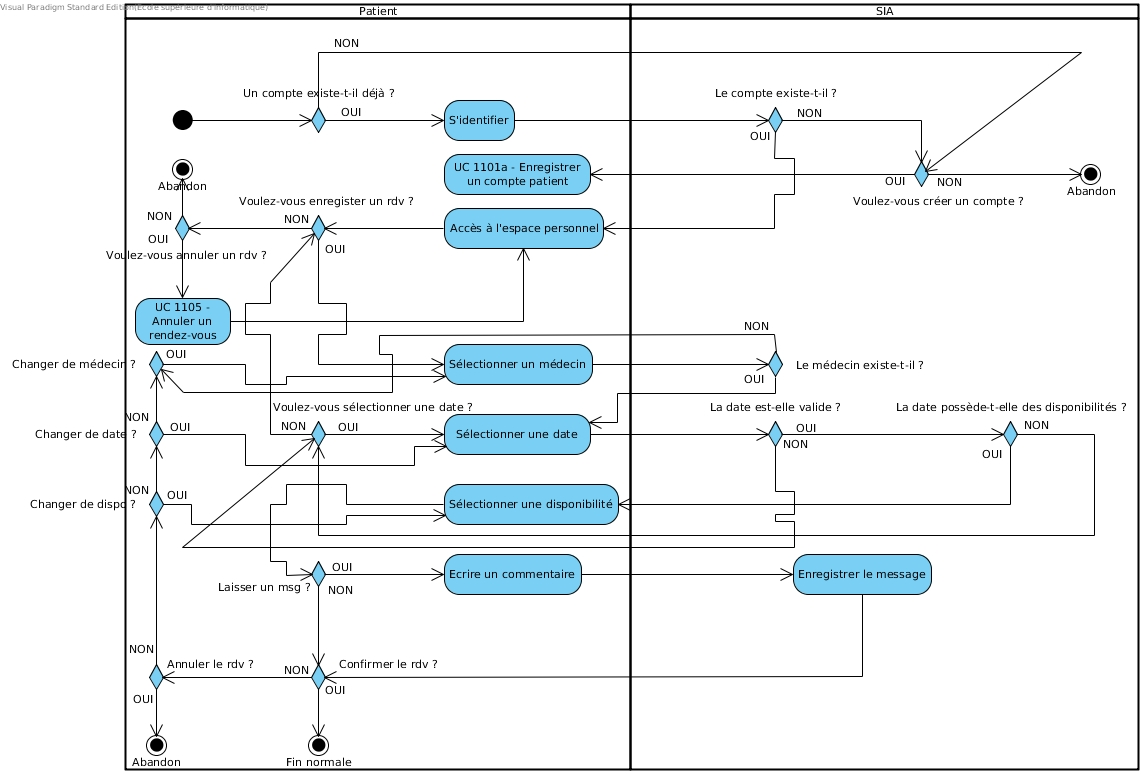
\includegraphics[scale=0.4]{MCT/activiteUC1104.jpg}
	\caption{Diagramme d'activité : \texttt{U.C. 1104}}
	\label{fig:act1104}
\end{figure}
\newpage

\section{Interface utilisateur}
\subsection{Exigences spéciales}
\texttt{S.O.}
\subsection{Aspect}
\begin{figure}[hb]
	\centering
	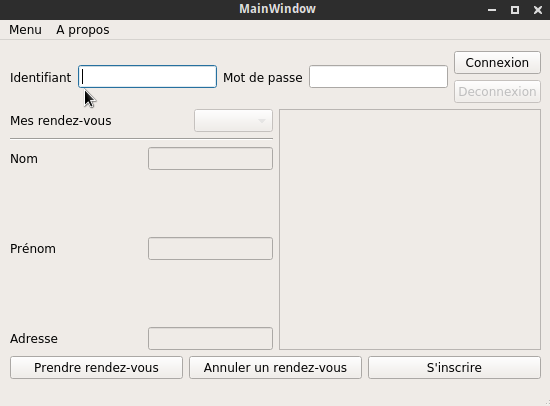
\includegraphics[scale=0.4]{MCT/GUI/workspace.png}
	\caption{Workspace}
	\label{fig:workspace}
\end{figure}
\begin{figure}[hb]
	\centering
	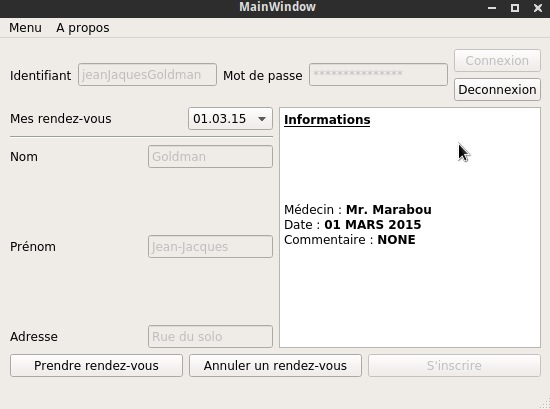
\includegraphics[scale=0.4]{MCT/GUI/connected.png}
	\caption{Workspace connecté}
	\label{fig:wrkconnected}
\end{figure}
\begin{figure}[hb]
	\centering
	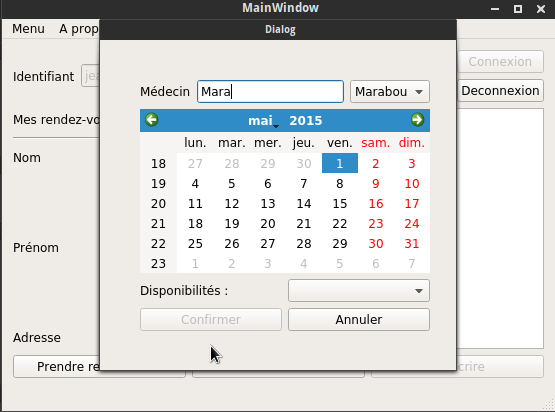
\includegraphics[scale=0.4]{MCT/GUI/rdv.png}
	\caption{Prise de rendez-vous}
	\label{fig:rdv}
\end{figure}
\begin{figure}[hb]
	\centering
	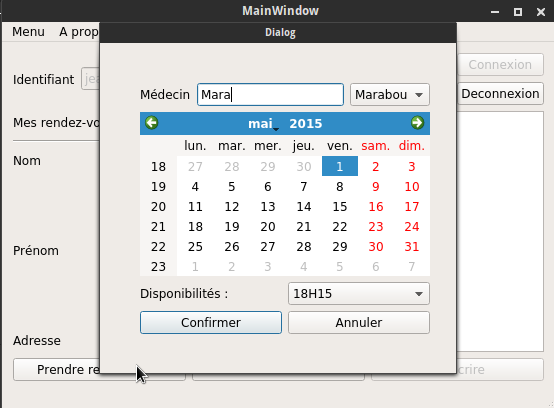
\includegraphics[scale=0.4]{MCT/GUI/rdvConfirm.png}
	\caption{Confirmation de rendez-vous}
	\label{fig:rdvConfirm}
\end{figure}
\newpage
\subsection{Règles de contrôle}
\texttt{Non demandé}


\chapter{Spécification \texttt{Use Case 1106} - Envoyer une notification}

\section{Introduction}

\subsection{Objectifs de ce document}

Ce document présente les spécifications fonctionnelles du \texttt{U.C. 1106} - Envoyer une notification.

\subsection{Domaine de définition de ce document}

\section{Définition du Use Case}

\subsection{Identifiant et nom}

\texttt{U.C. 1106} - Envoyer une notification.

\subsection{Brève description}

Avant un rendez-vous, le système envoie un rappel au patient pour le prévenir d'un rendez-vous.
Le patient peut choisir le temps avant le rendez-vous pour envoyer le rappel ainsi que le moyen
de communication (e-mail, sms, etc.).

\section{Flux}

\subsection{Flux de base}

Cet \texttt{U.C.} est déclenché automatiquement un certain nombre d'heure avant un rendez-vous. Quand un patient ou un médecin
définissent un rendez-vous, un envoi de notification est programmé. L'heure est
définie grâce aux paramètres utilisateur, de même
pour le type d'envoi. Le patient peut annuler un rendez-vous, si le rendez-vous est annulé alors que la notification est déjà
programmée, la notification est annulée et une nouvelle notification confirmant
l'annulation est envoyée directement au 
patient.

\subsection{Flux alternatif}

\subsubsection{Interruption du \texttt{U.C.}}

Si le système subit une panne, il faudra contacter l'administrateur système.
Celui-ci lancera un \texttt{U.C.} pour relancer les notifications non envoyées avec un message d'excuse accompagnant ces
notifications.


\section{Acteurs, mode, etc.}

\subsection{Acteurs}

Le S.I.A.\footnote{Système d'information automatisé} est l'acteur principale, 
c'est à dire qu'en cas de panne, il faudra s'adresser au responsable du système.

\subsection{Mode}

Automatisé unitaire.

\subsection{Évènement déclencheur}

Après que le patient ou le médecin ait créé un rendez-vous à l'aide du \texttt{U.C. 1104}. 
Un envoi de notification est programmé à une certaine heure avant l'heure du rendez-vous selon les 
paramètres utilisateur du patient.

\section{Pré-conditions}

Le patient doit avoir un rendez-vous de prévu.

\section{Post-conditions}

Aucune.

\section{Point d'inclusions et d'extensions}

S.O. (Sans Objets).
\section{Règles de gestion}

\subsection{Classes concernées}

La classe Rendez-vous et Compte Patient sont concernées en lecture seulement.

\subsection{Validation des encodages de données}

Aucune donnée n'est transmise de cette manière au système.

\subsection{Validation des données en sortie}

Aucune donnée transmise par le système ne nécessite une telle vérification.

\section{Diagramme d'activité}

Ce \texttt{U.C.} ne possède pas de diagramme d'activité, il est du ressort du système d'agir en fonction
des choix de l'utilisateur.

\section{Interface utilisateur}

Etant un \texttt{U.C.} automatisé, cet \texttt{U.C.} ne possède pas d'interface graphique.



\documentclass[a4paper, 11pt]{report}

\usepackage[utf8]{inputenc}                                                      
\usepackage[french]{babel}                                                       
\usepackage[T1]{fontenc}  
\usepackage[pdftex]{graphicx}                                                    
\usepackage{url}                                                                 
\usepackage{longtable}
\usepackage[bookmarks, colorlinks=false, pdfborder={0 0 0},
	pdftitle={Medicagenda}, 
	pdfauthor={Knop Florian, Kriwin Paul, Placentino Simon},
	pdfsubject={Medicagenda},           
pdfkeywords={UML, ISO/IEC 19505-1:2012, Medicagenda, Projet, analyse, ESI}]{hyperref}   

\newcommand{\HRule}{\rule{\linewidth}{0.5mm}}    

\begin{document}
\begin{titlepage}
	\begin{center}

		
\includegraphics[keepaspectratio=true,width=0.20\textwidth]{../ressources/logo}\\[1cm]

		\textsc{\LARGE H.E.B. Ecole Superieur d'Informatique}\\[1.5cm]

		\textsc{\Large Laboratoire d'analyse : Projet d'analyse}\\[0.5cm]
		\textsc{\Large Plan de tests fonctionnels élémentaires - UC 1104 -
		Définir un rendez-vous}\\[0.5cm]

		\HRule \\[0.4cm]
		{\huge \bfseries Medicagenda \\[0.4cm]}
		\HRule \\[1.5cm]

		\noindent
		\begin{minipage}[t]{0.4\textwidth}
			\begin{flushleft} \large
				\emph{Auteurs:}\\
				Florian \textsc{Knop} \href{mailto:39310@heb.be}{39310@heb.be}\\
				Paul \textsc{Kriwin} \href{mailto:39171@heb.be}{39171@heb.be}\\
				Simon \textsc{Placentino} \href{mailto:39631@heb.be}{39631@heb.be}\
			\end{flushleft}
		\end{minipage}%
		\begin{minipage}[t]{0.4\textwidth}
			\begin{flushright} \large
				\emph{Titulaire du cours:} \\
				Mr.~Nicolas \textsc{Pettiaux}
				\href{mailto:npettiaux@heb.be}{npettiaux@heb.be}
			\end{flushright}
		\end{minipage}

		\vfill

		{\large \today}

	\end{center}
	\clearpage\null\newpage
\end{titlepage}

\tableofcontents
\chapter{Plan de test fonctionnels élémentaires \texttt{U.C. 1104}}
\section{Introduction}
\subsection{Objectifs du document}
du document Ce document présente  le plan des tests fonctionnels du \texttt{U.C. 1104} -
définir un rendez-vous. 
\subsection{Domaine de définition du document}
Ce document ne présente que les scénarios correspondant à la définition d’un
rendez-vous (correspondant au diagramme d’activités de la description fonctionnelle
du UC).
\subsection{Définitions, acronymes et abréviations}
Définition INAMI : voir étude de cas et MCD\footnote{\href{../MCD/MCD.pdf}{voir document M.C.D.}}.
\subsection{Références}
\begin{itemize}
	\item[] Étude de cas de l'agenda
		médical\footnote{\href{../Enonce_Travail_Synthese_14-15.pdf}{voir
		étude de cas}}
	\item[] M.C.D. de \texttt{Medicagenda}\footnote{\href{../MCD/MCD.pdf}{voir document M.C.D.}}
	\item[] M.C.T. de \texttt{Medicagenda}\footnote{\href{./MCT.pdf}{voir document M.C.T.}}
	\item[] Spécifications fonctionnelles du \texttt{U.C.
		1104}\footnote{\href{./specifications_fonctionnelles_UC_1104_definir_un_rendez-vous.pdf}{Voir
			spécifications fonctionnelles du \texttt{U.C. 1104}}}
	\end{itemize}

	\paragraph{Remarque}
	dans le plan de test, il est prévu de faire appel aux UC 1101a/b – enregistrer un compte
	patient/médecin ainsi qu'à l'\texttt{U.C. 1103} - définir une disponibilité.
	Les \texttt{U.C. 1101a/b} et \texttt{1103} devront
	donc être réalisé et testé avant le présent \texttt{U.C. 1104}.

	\section{Types de tests élémentaires fonctionnels}
	\subsection{Validation des règles de saisie}
	\textbf{UC interactif}
	Validation des formats et valeurs des champs: voir description de l’interface et
	des messages d’erreur liés à son utilisation.

	La date et heure du rendez-vous à réserver ne doivent pas être antérieurs au
	moment où a lieu la réservation. 
	\subsection{Validation des règles de calcul}
	\texttt{S.O.}
	\subsection{Validation des mises à jour du SI}
	Vérification de la création correcte des nouveaux enregistrements dans la base
	de données, pour les différents scénarios décrits ci-dessous, ainsi que des
	liens entre objets de classes différentes. 
	Cela implique que le nouveau rendez-vous créé concerne les bons comptes
	utilisateurs, est à la date et heure convenue et que la plage horaire occupée
	par celui-ci soit dorénavant indisponible.
	\subsection{Validation des outputs utilisateurs}
	Vérification que les messages d’erreurs et de validations apparaissent
	pertinemment et s’affichent correctement. Les messages de récapitulation de la
	réservation doivent être pertinents pour les deux types d’utilisateurs (médecin
	et utilisateur) et exempts de toutes erreurs.
	\subsection{Tests de consolidation}

	\subsection{Tests de saisie}
	\subsection{Cas extrêmes}
	Au cours de différents scénarios, tests de l'abandon du \texttt{U.C.} et vérification que
	la base de données est effectivement restée intacte.
	\section{Scénarios de tests}
	Scénario |   cas  |         description    |   Résultat attendu 

	\begin{itemize}
		\item[] \texttt{scénario 0. cas 1.} 
			\begin{itemize}
				\item description: \\
					Le patient possède déjà un compte, a sélectionné un médecin ou une date ou une
					plage horaire mais désire annuler son choix pour en sélectionner un/une autre.
				\item résultat:\\
					La base de donnée n’est jamais modifiée, et la fenêtre de l’étape précédente
					est réaffichée.\\
			\end{itemize}
		\item[] \texttt{scénario 1. cas 1.1}
			\begin{itemize}
				\item description:  \\
					Le patient possède déjà un compte, a sélectionné et validé
					un médecin et une date et heure disponible.
				\item résultat: \\
					un fenêtre affiche le calendrier et la barre de recherche
					pour entrer le nom du medecin. 
					Une fois ce dernier et une date valide séléctionnés, est
					affichée une grille horaire de cette date avec les
					disponibilités du médecin. Après que la plage horraire eu
					été séléctionnée, 
					le message récapitulatif de la réservation s’est affiché et
					a été validé. 
					Le nouveau rendez-vous est enregistré, il s’affiche dans le
					calendrier du patient et dans celui du médecin, la
					disponibilité correspondant à la plage horaire du nouveau
					rendez-vous n’est plus.\\
			\end{itemize}
		\item[] \texttt{scénario 1. cas 1.2}
			\begin{itemize}
				\item description:  \\
					idem que 1.1 mais le patient n’est pas enregistré
				\item résultat: \\
					idem que 1.1 mais le patient s’ enregistre au préalable
					(appel au \texttt{U.C. 1101})\\
			\end{itemize}
		\item[] \texttt{scénario 2. cas 2.1}
			\begin{itemize}
				\item description:\\
					Le patient sélectionne un médecin et essaye de sélectionner
					une date ne contenant pas de disponibilité.
				\item résultat: \\
					Statu quo, les dates concernées doivent êtres non cliquable
					et rien ne doit alors se passer.\\
			\end{itemize}
		\item[] \texttt{scénario 2. cas 2.2}
			\begin{itemize}
				\item description:\\
					Le patient sélectionne un médecin et essaye de sélectionner
					une date antérieure au moment de la réservation.
				\item résultat: \\
					Idem que 2.1.\\
			\end{itemize}
		\item[] \texttt{scénario 2. cas 2.3}
			\begin{itemize}
				\item description:\\
					Le patient sélectionne un médecin et essaye de sélectionner
					une date à laquelle le médecin possède des disponibilités,
					mais une plage horaire à laquelle il possède déjà un
					rendez-vous.
				\item résultat: \\
					statu quo, les cases représentant ces disponibilités
					doivent être rougie avec un message décrivant le fait que le
					patient a déjà un rendez vous à ce moment là et donc,
					doivent êtres non cliquable et rien ne doit alors se passer.\\
			\end{itemize}
	\end{itemize}
	\newpage
	\section{Valeurs}
	\subsection{Valeurs d'initialisation}
	Pour pouvoir faire les tests des scénarios 1 et 2, il faudra disposer d’une
	base de données contenant un nombre minimal de comtes médecins avec
	disponibilités, ainsi que de quelques comptes patients.
	Il faudra également disposer du \texttt{U.C. 1101} testé qui peut être appelé par le
	présent \texttt{U.C. 1104}.
	\subsection{Valeurs spécifiques}
	Avant les tests, il faut constituer la base de données de tests et des cas
	de tests avec des disponibilités et rendez-vous déjà présents dans les
	calendrier des médecins et patients (ne pas oublier que l'environnement de
	tests (comme l'environnement de développement) doit être séparé de
	l'environnement de production).
	Les données spécifiques se retrouveront dans la base de données qui sera
	mise à la disposition des testeurs. Pour ``peupler'' cette base de données, il
	sera fait appel à des outils d’encodage rapide de données.
	\end{document}

\chapter{Plan de test fonctionnels élémentaires \texttt{U.C. 1106}}
\section{Introduction}
\subsection{Objectifs du document}
Ce document présente le plan des tests fonctionnels du \texttt{U.C. 1106} -
envoyer une notification. 
\subsection{Domaine de définition du document}
Ce document ne présente que les scénarios correspondant à l'envoi d’une
notification (correspondant au diagramme d’activités de la description 
fonctionnelle du \texttt{U.C.}).
\subsection{Définitions, acronymes et abréviations}
Définition INAMI : voir étude de cas et MCD\footnote{\href{../MCD/MCD.pdf}{voir document M.C.D.}}.
\subsection{Références}
\begin{itemize}
	\item[] Étude de cas de l'agenda
		médical\footnote{\href{../Enonce_Travail_Synthese_14-15.pdf}{voir
		étude de cas}}
	\item[] M.C.D. de \texttt{Medicagenda}\footnote{\href{../MCD/MCD.pdf}{voir document M.C.D.}}
	\item[] M.C.T. de \texttt{Medicagenda}\footnote{\href{./MCT.pdf}{voir document M.C.T.}}
	\item[] Spécifications fonctionnelles du \texttt{U.C.
		1106}\footnote{\href{./specifications_fonctionnelles_UC_1106_envoyer_une_notification.pdf}{Voir
			spécifications fonctionnelles du \texttt{U.C. 1106}}}
	\end{itemize}

	\section{Types de tests élémentaires fonctionnels}
	\subsection{Validation des règles de saisie}
	Aucune car il n’existe pas d’interface dans un \texttt{U.C.} automatisé.
	\subsection{Validation des règles de calcul}
	\texttt{S.O.}
	\subsection{Validation des mises à jour du SI}
	Aucune, ce \texttt{U.C.} accède à la base de donnée uniquement lecture.
	\subsection{Validation des outputs utilisateurs}
	Validation du contenu et de l'affichage des messages de notification. 
	Ces derniers doivent être exempts d’erreurs au sein de leurs contenus et
	garantir qu'ils sont adressés au bon patient pour le bon rendez-vous.
	\subsection{Tests de consolidation}
	Tous les scénarios peuvent commencer par un encodage de données à 
	vérifier par l'interface.;
	\subsection{Tests de saisie}
	Aucuns, il s’agit d’un \texttt{U.C.} automatisé.
	\subsection{Cas extrêmes}
	Vérification des message en cas de relance du SI après une panne.
	\section{Scénarios de tests}
	\begin{itemize}
		\item[] \texttt{scénario 1. Cas 1.1}
			\begin{itemize}
				\item description:  \\
					Le patient possède un rendez-vous pour le lendemain, a fixé
					la notification à 18h la veille du rendez-vous et comme
					format de notification, l'email.
				\item résultat: \\
					A 18h doit être reçu sur la boîte email du patient, le
					message de notification indiquant le temps restant avant le
					rendez-vous et les informations inhérentes à celui-ci.
			\end{itemize}
		\item[] \texttt{scénario 1. Cas 1.2}
			\begin{itemize}
				\item description:  \\
					Idem que 1.1, avec la notification par SMS définie en plus. 
				\item résultat: \\
					Idem que 1.1 avec la réception au même moment d’un autre
					message de notification sur la boîte SMS du patient
			\end{itemize}
		\item[] \texttt{scénario 2. Cas 2.1}
			\begin{itemize}
				\item description:\\
					Idem que 1.2 sauf que quelques heures avant la notification
					prévue, le patient annule son rendez-vous.
				\item résultat: \\
					Le patient ne doit alors pas être notifié quand viendra
					l'heure de la notification du rendez-vous avorté. 
					Mais peu après avoir programmé l'annulation du rendez-vous,
					doit à la place, recevoir une notification de confirmation
					d’annulation.
			\end{itemize}
		\item[] \texttt{scénario 3. Cas 3.1}
			\begin{itemize}
				\item description:\\
					une panne du SI survient.
				\item résultat: \\
					Lors de la remise en marche de celui-ci, les notifications
					non envoyées à cause de la panne, doivent être complétées
					par un message d’excuse expliquant le problème technique
					survenu.
			\end{itemize}
	\end{itemize}
	\newpage
	\section{Valeurs}
	\subsection{Valeurs d'initialisation}
	Il faudra définir à chaque fois tous les enregistrements des tables de la
	base de données. 
	Ceci donnera lieu à des programmes de génération de données, et des 
	programmes permettant de faire évoluer les dates système.
	\subsection{Valeurs spécifiques}
	A définir au moment des tests.


\end{document}
